%%%%%%%%%%%%%%%%%%%%%%%%%%%%%%%%%%%%%%%%%%%%%%%%%%%%%%%%%%%%%%%%%%%%%%%%%%%%%%%%
%2345678901234567890123456789012345678901234567890123456789012345678901234567890
%        1         2         3         4         5         6         7         8

\documentclass[letterpaper, 10 pt, conference]{ieeeconf}  % Comment this line out if you need a4paper

%\documentclass[a4paper, 10pt, conference]{ieeeconf}      % Use this line for a4 paper

\IEEEoverridecommandlockouts                              % This command is only needed if 
                                                          % you want to use the \thanks command

\overrideIEEEmargins                                      % Needed to meet printer requirements.

%In case you encounter the following error:
%Error 1010 The PDF file may be corrupt (unable to open PDF file) OR
%Error 1000 An error occurred while parsing a contents stream. Unable to analyze the PDF file.
%This is a known problem with pdfLaTeX conversion filter. The file cannot be opened with acrobat reader
%Please use one of the alternatives below to circumvent this error by uncommenting one or the other
%\pdfobjcompresslevel=0
%\pdfminorversion=4

% See the \addtolength command later in the file to balance the column lengths
% on the last page of the document

% The following packages can be found on http:\\www.ctan.org
\usepackage{graphics} % for pdf, bitmapped graphics files
\usepackage{epsfig} % for postscript graphics files
\usepackage{cite}
%\usepackage{mathptmx} % assumes new font selection scheme installed
%\usepackage{times} % assumes new font selection scheme installed
%\usepackage{amsmath} % assumes amsmath package installed
%\usepackage{amssymb}  % assumes amsmath package installed




\title{\LARGE \bf
 Local network coordination supports neuroprosthetic control
}


\author{William Liberti III$^{1}$, Xue Lily Gong$^{2}$, Thomas Roseberry$^{3}$, and Jose Carmena$^{4}$, \emph{Senior Member, IEEE}% <-this % stops a space
%\thanks{*This work was not supported by any organization}% <-this % stops a space
\thanks{$^{1}$William Liberti is a Fellow in the Department of Electrical Engineering and Computer Science, U.C. Berkeley, Berkeley, CA 94708, USA
        {\tt\small bliberti@bu.edu}}%
\thanks{$^{2}$Lily Xue Gong is a Graduate Student in the Helen Wills Neuroscience Institute, U.C. Berkeley, Berkeley, CA 94708, USA}
\thanks{$^{3}$Thomas Roseberry is an engineer at Neuralink, San Francisco, CA 94708, USA}
        %{\tt\small bliberti@bu.edu}}%
\thanks{$^{4}$Jose Carmena is a full professor in the Department of Electrical Engineering and Computer Science, U.C. Berkeley, Berkeley, CA 94708, USA
        {\tt\small jcarmena@berkeley.edu}}%
}


\begin{document}



\maketitle
\thispagestyle{empty}
\pagestyle{empty}


%%%%%%%%%%%%%%%%%%%%%%%%%%%%%%%%%%%%%%%%%%%%%%%%%%%%%%%%%%%%%%%%%%%%%%%%%%%%%%%%
\begin{abstract}

Learning often involves adapting behavior in response to the inferred causes of success and failure. At the neural level, this can be the result of repeating activity patterns of neurons that lead to favorable outcomes. However, it is not clear how networks assess the contributions of individual cells to an ongoing behavior. Using a calcium imaging based closed loop Brain Machine Interface (BMI), we trained mice to perform a neuroprosthetic task using the coordinated activity of a small ensemble of neurons in layer 2/3 of sensorimotor cortex. Throughout a single 30 minute session, network conformations that result in reward dramatically increase in frequency relative to similar conformations in other cells. We find that that after an initial period of exploration, neurons unrelated to the task demonstrate a decrease in variance and event frequency over the course of learning. However, many of these `indirect' cells demonstrate robust spatiotemporal dynamics both before and after an animal achieves reward. We estimate the relative contributions of the local network by using nearby, unrelated cells to decode the activity of the BMI neurons compared to arbitrary neurons uninvolved with this task. Taken together, our findings suggest that neuroprosthetic control of output cells is the result of specific spatiotemporal ensemble patterns that are quickly identified and reinforced.




\end{abstract}


%%%%%%%%%%%%%%%%%%%%%%%%%%%%%%%%%%%%%%%%%%%%%%%%%%%%%%%%%%%%%%%%%%%%%%%%%%%%%%%%
\section{INTRODUCTION}


Several studies of learning have shown that spatiotemporal activity patterns of neurons which lead to desired behavioral outcomes are selected and consolidated \cite{Fetz1969-pt,Ganguly2009-qy,Athalye2018-lo}. The theoretical framework that describes this underlying computational problem is called `credit assignment', and it is an important ingredient of reinforcement learning \cite{Sutton1998-bm}. However, the single neuron rules that result in behavior modification or maintenance have been difficult to address, due to the immense fine-scale complexity of biological neural networks and the heterogeneity of natural behavior. Traditional behavioral assays are agnostic to the underlying neural dynamics used by animals to accomplish a given task, making it nearly impossible to assert the causal role of individual neurons to a behavioral action. Moreover, natural tasks are thought to engage hundreds of thousands of neurons; most of these elements are unobservable to the experimenter, making it impossible to estimate the redundancy and degeneracy of neural codes that coordinate learned skills. With current technology, a holistic understanding of the single unit code that underlies natural skill learning is an under-constrained problem.

 To overcome these obstacles, we employ a reductionist approach where the behavioral output is simply the optically recorded activity of a small ensemble of experimenter defined cortical neurons expressing genetically encoded fluorescent calcium indicators. This neuroprosthetic strategy uses closed-loop auditory feedback to guide a `fictive behavior' where animals are rewarded when a specific network conformation is observed in a chosen neural population \cite{Clancy2014-ju,Grosenick2015-hy}. Similar to natural motor tasks, previous work has shown that neuroprosthetic task performance tends to increases over days \cite{Clancy2014-ju}. Surprisingly, BMI performance can increase even when the output cell identity is changed from day to day-  suggesting that mice are learning to better assign reward credit to output neurons, rather than consolidating specific activity control patterns \cite{Peters2014-xd,Gulati2017-rz,Mitani2018-rp}. It is unclear how the local population of cells resolves the identity of the output cells on these short timescales.  The remaining units that are not assigned a direct relationship with effector, called  \emph{`indirect neurons'}, do demonstrate some tuning relative to BMI tasks, suggesting that some these neurons also become incorporated into functional neuronal assemblies that help coordinate neurons that directly drive output \cite{Prsa2017-rn,Ganguly2011-je}. However, limited cell yields from chronic electrophysiology and an experimenter bias to assign the highest signal-to-noise units as output cells has provided limited opportunities to ask questions about the relative contributions of local networks \cite{Ganguly2011-je}.


After an initial period of exploration, we find that the local cortical neural population converges to form reproducible, spatiotemporally organized activity patterns that increases in frequency and robustness through a 30 minute session \cite{Clancy2014-ju,Prsa2017-rn}. Our findings suggest that neuroprosthetic control can be the result of an emergent, spatially organized network level solution.





\section{METHODS}
\subsection{Animals and Surgical Procedure.}
All animal procedures were performed in accordance with U.C. Berkeley IACUC regulations. Stereotactic surgery was performed in (n=5)  $Emx1^{IRES cre }$ or wild type mice as previously described \cite{Clancy2014-ju}. 200-300nl of AAV2.9 CamKII.GCamp6f.WPRE.SV40 or AAV5-SYN-FLEX-GCaMP6f-WPRE-SV40 was used to preferentially label excitatory cells in cortex. Mice were given 4 weeks post-surgical recovery time to allow for sufficient protein expression.
  \begin{figure}[thpb]
      \centering
%      \framebox{\parbox{3in}{We suggest that you use a text box to insert a graphic (which is ideally a 300 dpi TIFF or EPS file, with all fonts embedded) because, in an document, this method is somewhat more stable than directly inserting a picture. }}
      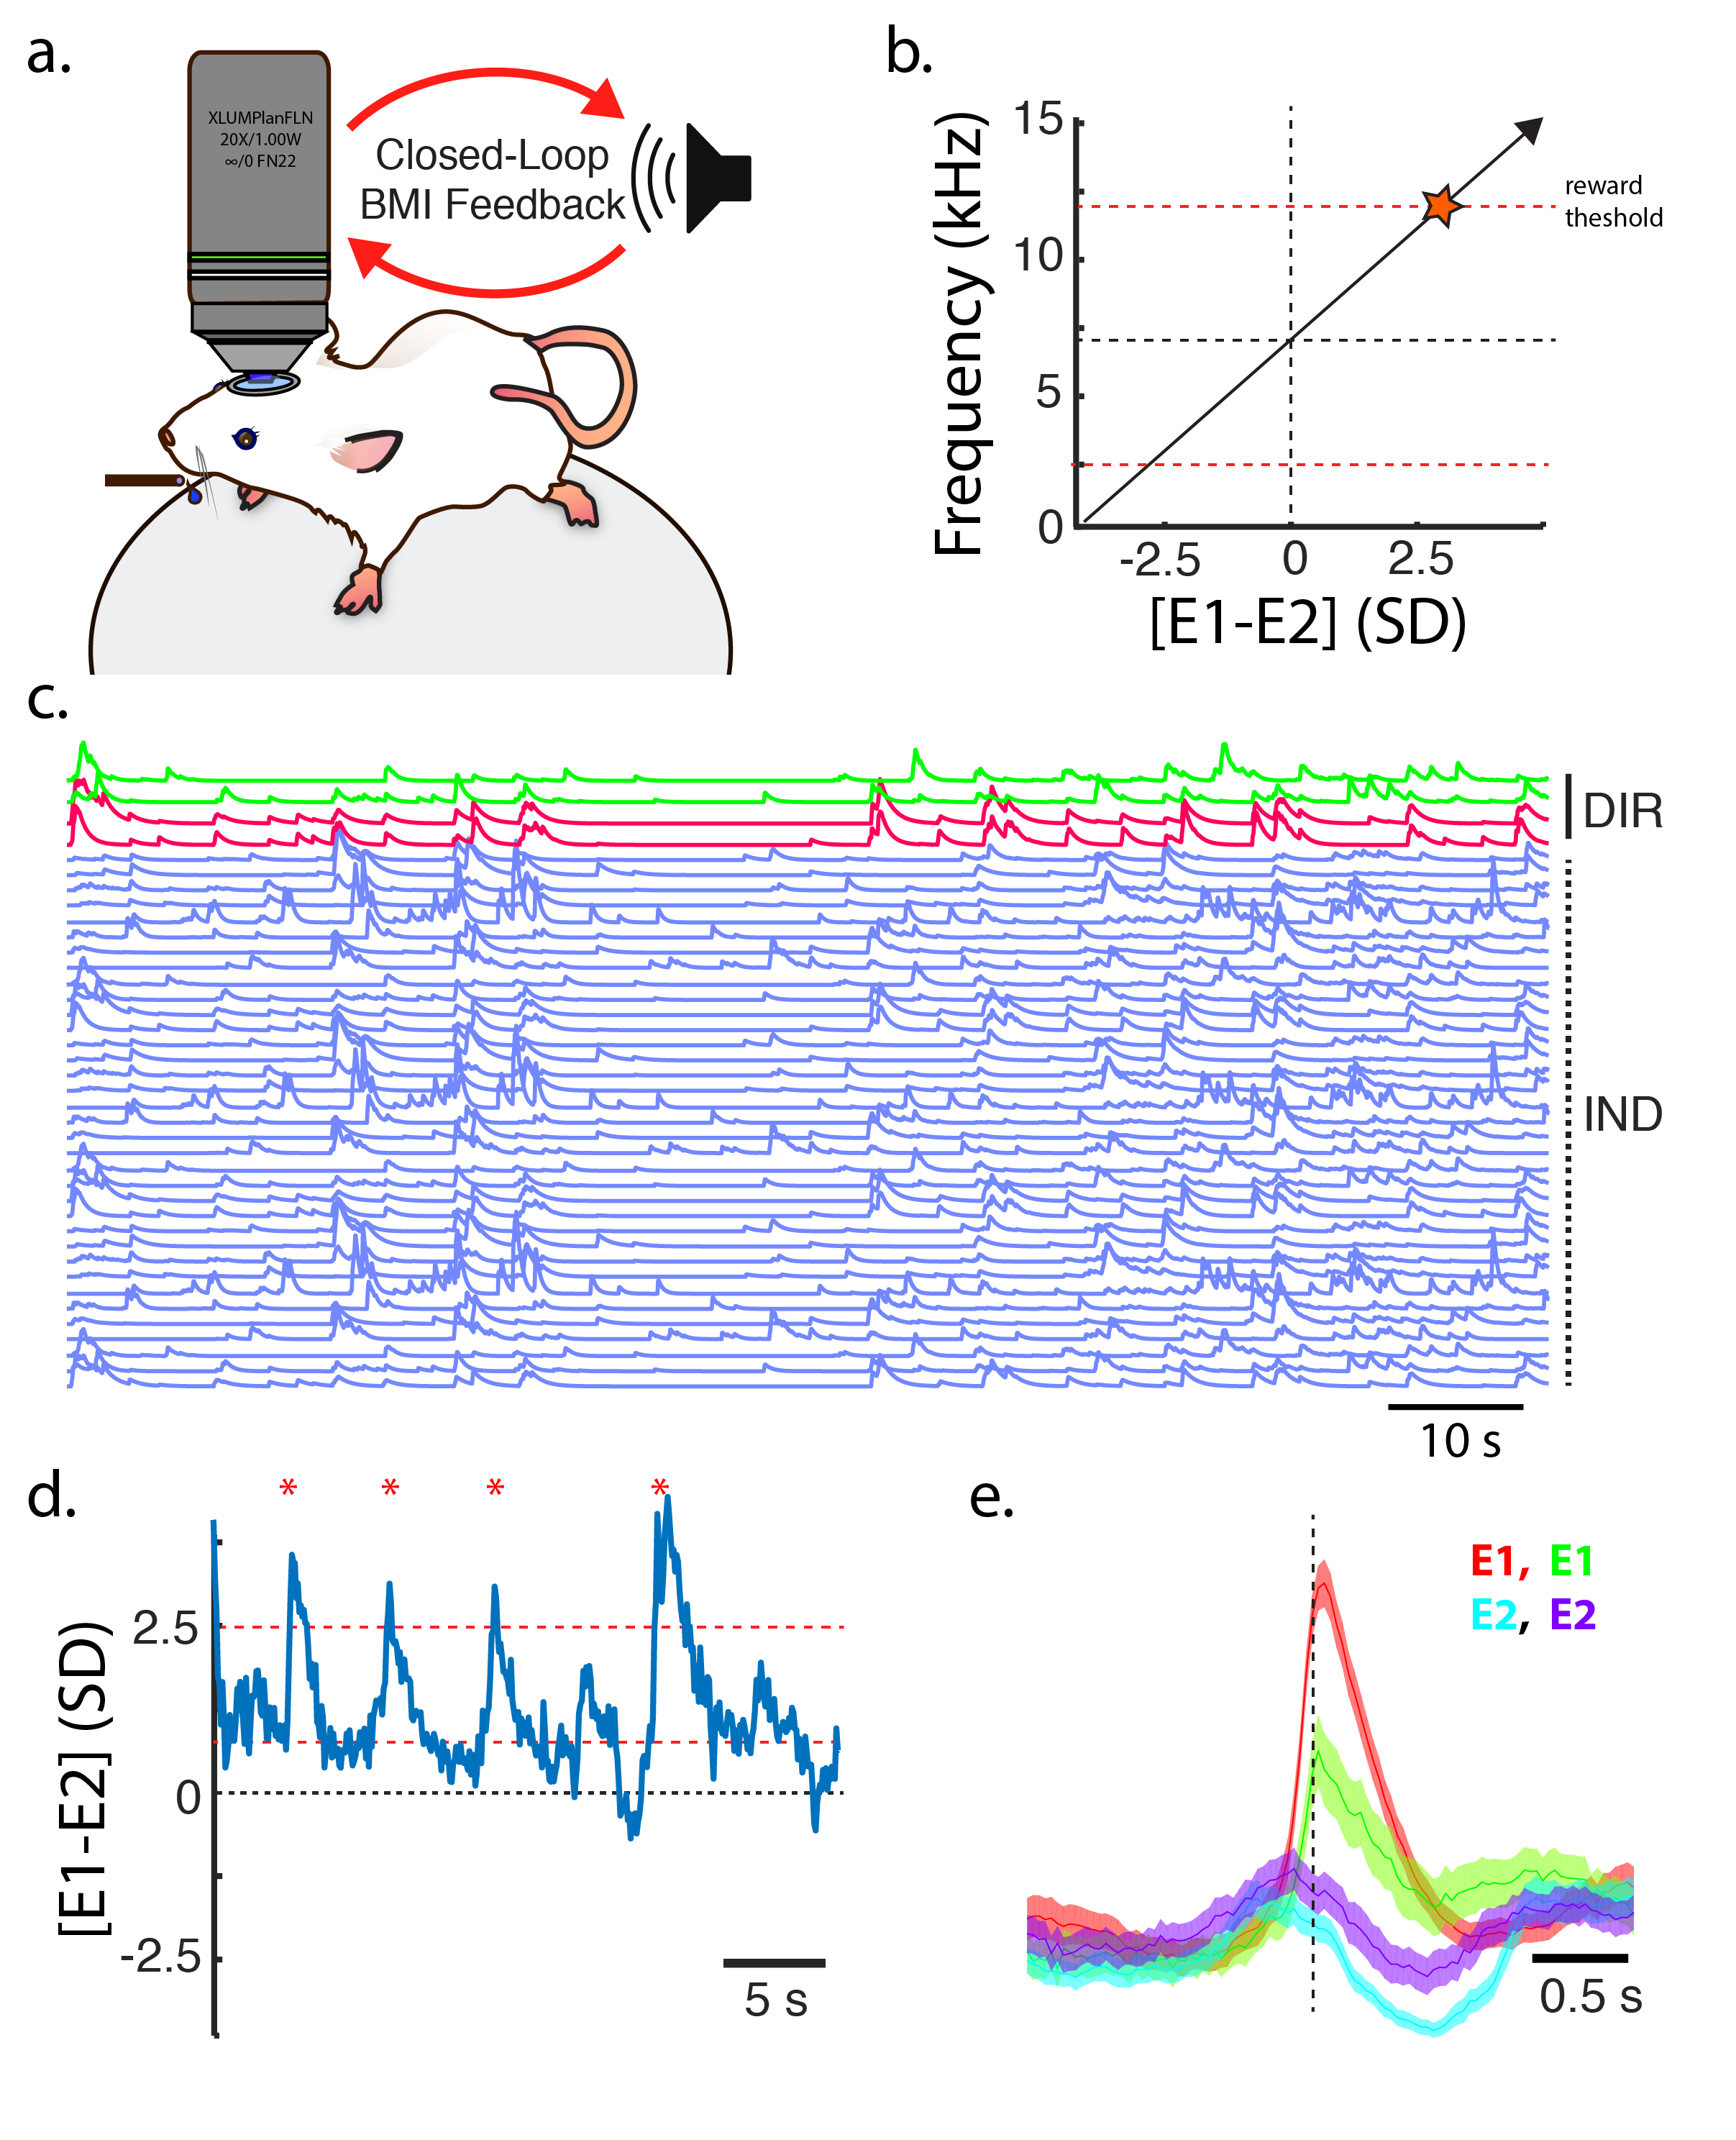
\includegraphics[scale=.38]{figures/figure01.png}
      \caption{\emph{Experimental paradigm for a closed-loop calcium imaging based auditory feedback.} $(A)$ Head-fixed mice run freely on a spherical treadmill, and perform BMI experiments for a water reward.  $(B)$  Mice must modulate calcium dynamics in neuronal ensembles to move a cursor to a high-pitched target tone that was associated with reward. ($C$) Two ensembles ( eg, $E1$ in green; $E2$ in red) of 2 single cells each were chosen for inclusion in the `direct' output population. We were able to observe hundreds of additional `indirect' neurons in the same field of view, their $\Delta F/F_{0}$ over time is schematized in blue. $(D)$  Mice were able to modulate the calcium dynamics in these neuronal ensembles to move a cursor 2.5$SD$ above baseline levels. Additional reward was prevented until the cursor returned to within baseline levels ( 1$SD$ of the mean). $(E)$  Output neuron activity converges to form reproducible activity patterns to achieve a reward. Shown here is the average $E1$ and $E2$ population centered at the hit. Shading represents  2x$sem$. }
      \label{figurelabel}
   \end{figure}

\subsection{Experimental Preparation}
In vivo imaging was performed at 30Hz using a commercial multi-photon microscope (Bruker, Ultima Investigator) driven by a mode-locked, tunable Ti:Sapphire laser (CHAMELEON ULTRA II) and set to 900-980 nm, steered via 8kHz resonant galvos through a 20x water immersion objective (XLUMPLFLN 20XW). Photons were collected with a GaAsP photomultiplier tube (Hamamatsu Model H10770). Mice were put on a restricted water regiment for the duration of the experiment \cite{Guo2014-db}. During the task, mice were head-fixed but allowed to run freely on a circular treadmill,  consisting of styrofoam ball suspended by air (PhenoSys, JetBall Virtual Reality System). Non-rigid image registration, ROI extraction, baseline de-trending, and spike deconvolution was performed offline. \cite{Pnevmatikakis2017-ch,Pnevmatikakis2016-bg}



\subsection{Behavioral Task}
The boundaries of two ensembles of two single cells were manually defined after a 3-15 minute baseline period of imaging. Care was taken to use well isolated regions of interest (ROIs).   Depending on the density of viral labeling, we were able to observe ~300-800 additional neurons in a 500$um^{2}$ field of view. Ensemble activity was measured as the summed, running z-score normalized $\Delta F/F_{0}$ for each component neuron. This normalization is performed  to scale each neuron by its dynamic range, in order to overcome potential differences in viral expression across cells, such that each direct unit would contributed equally to the output. The cursor was smoothed with a running average of 2 - 3 frames. Closed-loop latency was ~38ms, with a jitter  of ~17ms ( 95\% confidence). Frequencies used for auditory feedback ranged from 1-20 kHz in quarter-octave increments to match rodent psychophysical discrimination thresholds \cite{Clancy2014-ju}. Mice must modulate calcium dynamics in these neuronal ensembles to move the cursor to a high-pitched target tone that was associated with water reward, set at 2.5 standard deviations ($SD$) above the baseline (Fig 1b). Additional reward was prevented until the cursor returned to within baseline levels ( 1$SD$ of the cursor mean). 
\subsection{L2-regularized Linear Regression Model }

Indirect neuron features were derived from the spike deconvolved calcium activity within a 2 second sliding window [timepoints * spike and height features]. The response matrix consisted of the fluorescent change ($\Delta F/F_{0}$ ) of each direct neuron ($E1\textsubscript{a}$, $E1\textsubscript{b}$, $E2\textsubscript{a}$, $E2\textsubscript{b}$), the cursor ($E1-E2$), and the 2 ensembles $E1$ and $E2$.  We separated the indirect neuron feature matrix ($IND$) and direct neuron response matrix ($DN$) into a training dataset ($IDN: 54378 * 1580, DN: 54378 * 7$) and completely withheld validation dataset based at the moment of the `hit': ($IDN: 112 * 1580, DN: 112 * 7$).  To avoid bias, we fixed the regularization coefficient- determined by cross-validating the regression procedure 5$\times$. In each cross-validation iteration, 80\% of the training dataset was used to estimate the model weights for each of 10 possible regularization coefficients of the remaining 20\%. After the completion of cross-validation, a regularization-performance curve was obtained by averaging the cross-validation sample $R^2$ first across 10 regularization coefficients samples and then across all 7 direct neuron responses, then the best regularization parameter (21.544) was selected. Model estimated weights were used to predict responses of the withheld validation dataset.  We repeated the modeling procedure using the features of indirect neurons to predict shuffled direct neurons' response matrix in time (frames) axis. We shuffled the response matrix 1000$\times$  to build a null distribution of $R^2$ to obtain $P$ values\cite{Nunez-Elizalde2018-ia}.



\section{Results} 

\subsection{Evidence Against Solution Degeneracy}
	Mice were able to modulate the calcium dynamics in these neuronal ensembles to move the cursor to a high-pitched target tone that was associated with water reward (Fig 1c) \cite{Clancy2014-ju}. An increase in reward frequency could result from a non-specific, or a multitude of degenerate strategies, instead of specifically controlling individual cells. For example, upon hearing a tone, increased attention or arousal may increase unit excitability, increasing cortical network entropy compared to a baseline period. This feedback loop would increase the chance level of reward compared to baseline- and appear to be volitional control of individual cells \cite{Prsa2017-rn}.

	If this was true, we would expect that both the variance across the network, and the average number of events across individual cells in the interval immediately before the hit criteria is met would remain constant or increase over the course of the session, reflecting a strategy of using numerous state permutations to gain reward. However, we observe the opposite- total variance across the network tends to decrease over time, as does the mean population activity of indirect neurons in the moments leading up to the hit (Fig 2c-d). In contrast,  cells that are involved with the cursor increase their activity over the session at the moment of the hit (Fig 2a). Given these results, we reasoned that it would be appropriate to normalize the number of rewards over the session as a function of the number of rewards that would have been achieved if any other pairs of neurons had been driving the cursor. This would provide a control to see if the neural population consolidates a limited number of network conformations that earned a reward. Compared to the population, we find there is a strong trend to increase reward related conformations over time, supporting the notion that specific activity patterns are being consolidated on this timescale (Fig 2b). 



   \begin{figure}[thpb]
      \centering
%      \framebox{\parbox{3in}{We suggest that you use a text box to insert a graphic (which is ideally a 300 dpi TIFF or EPS file, with all fonts embedded) because, in an document, this method is somewhat more stable than directly inserting a picture. }}
      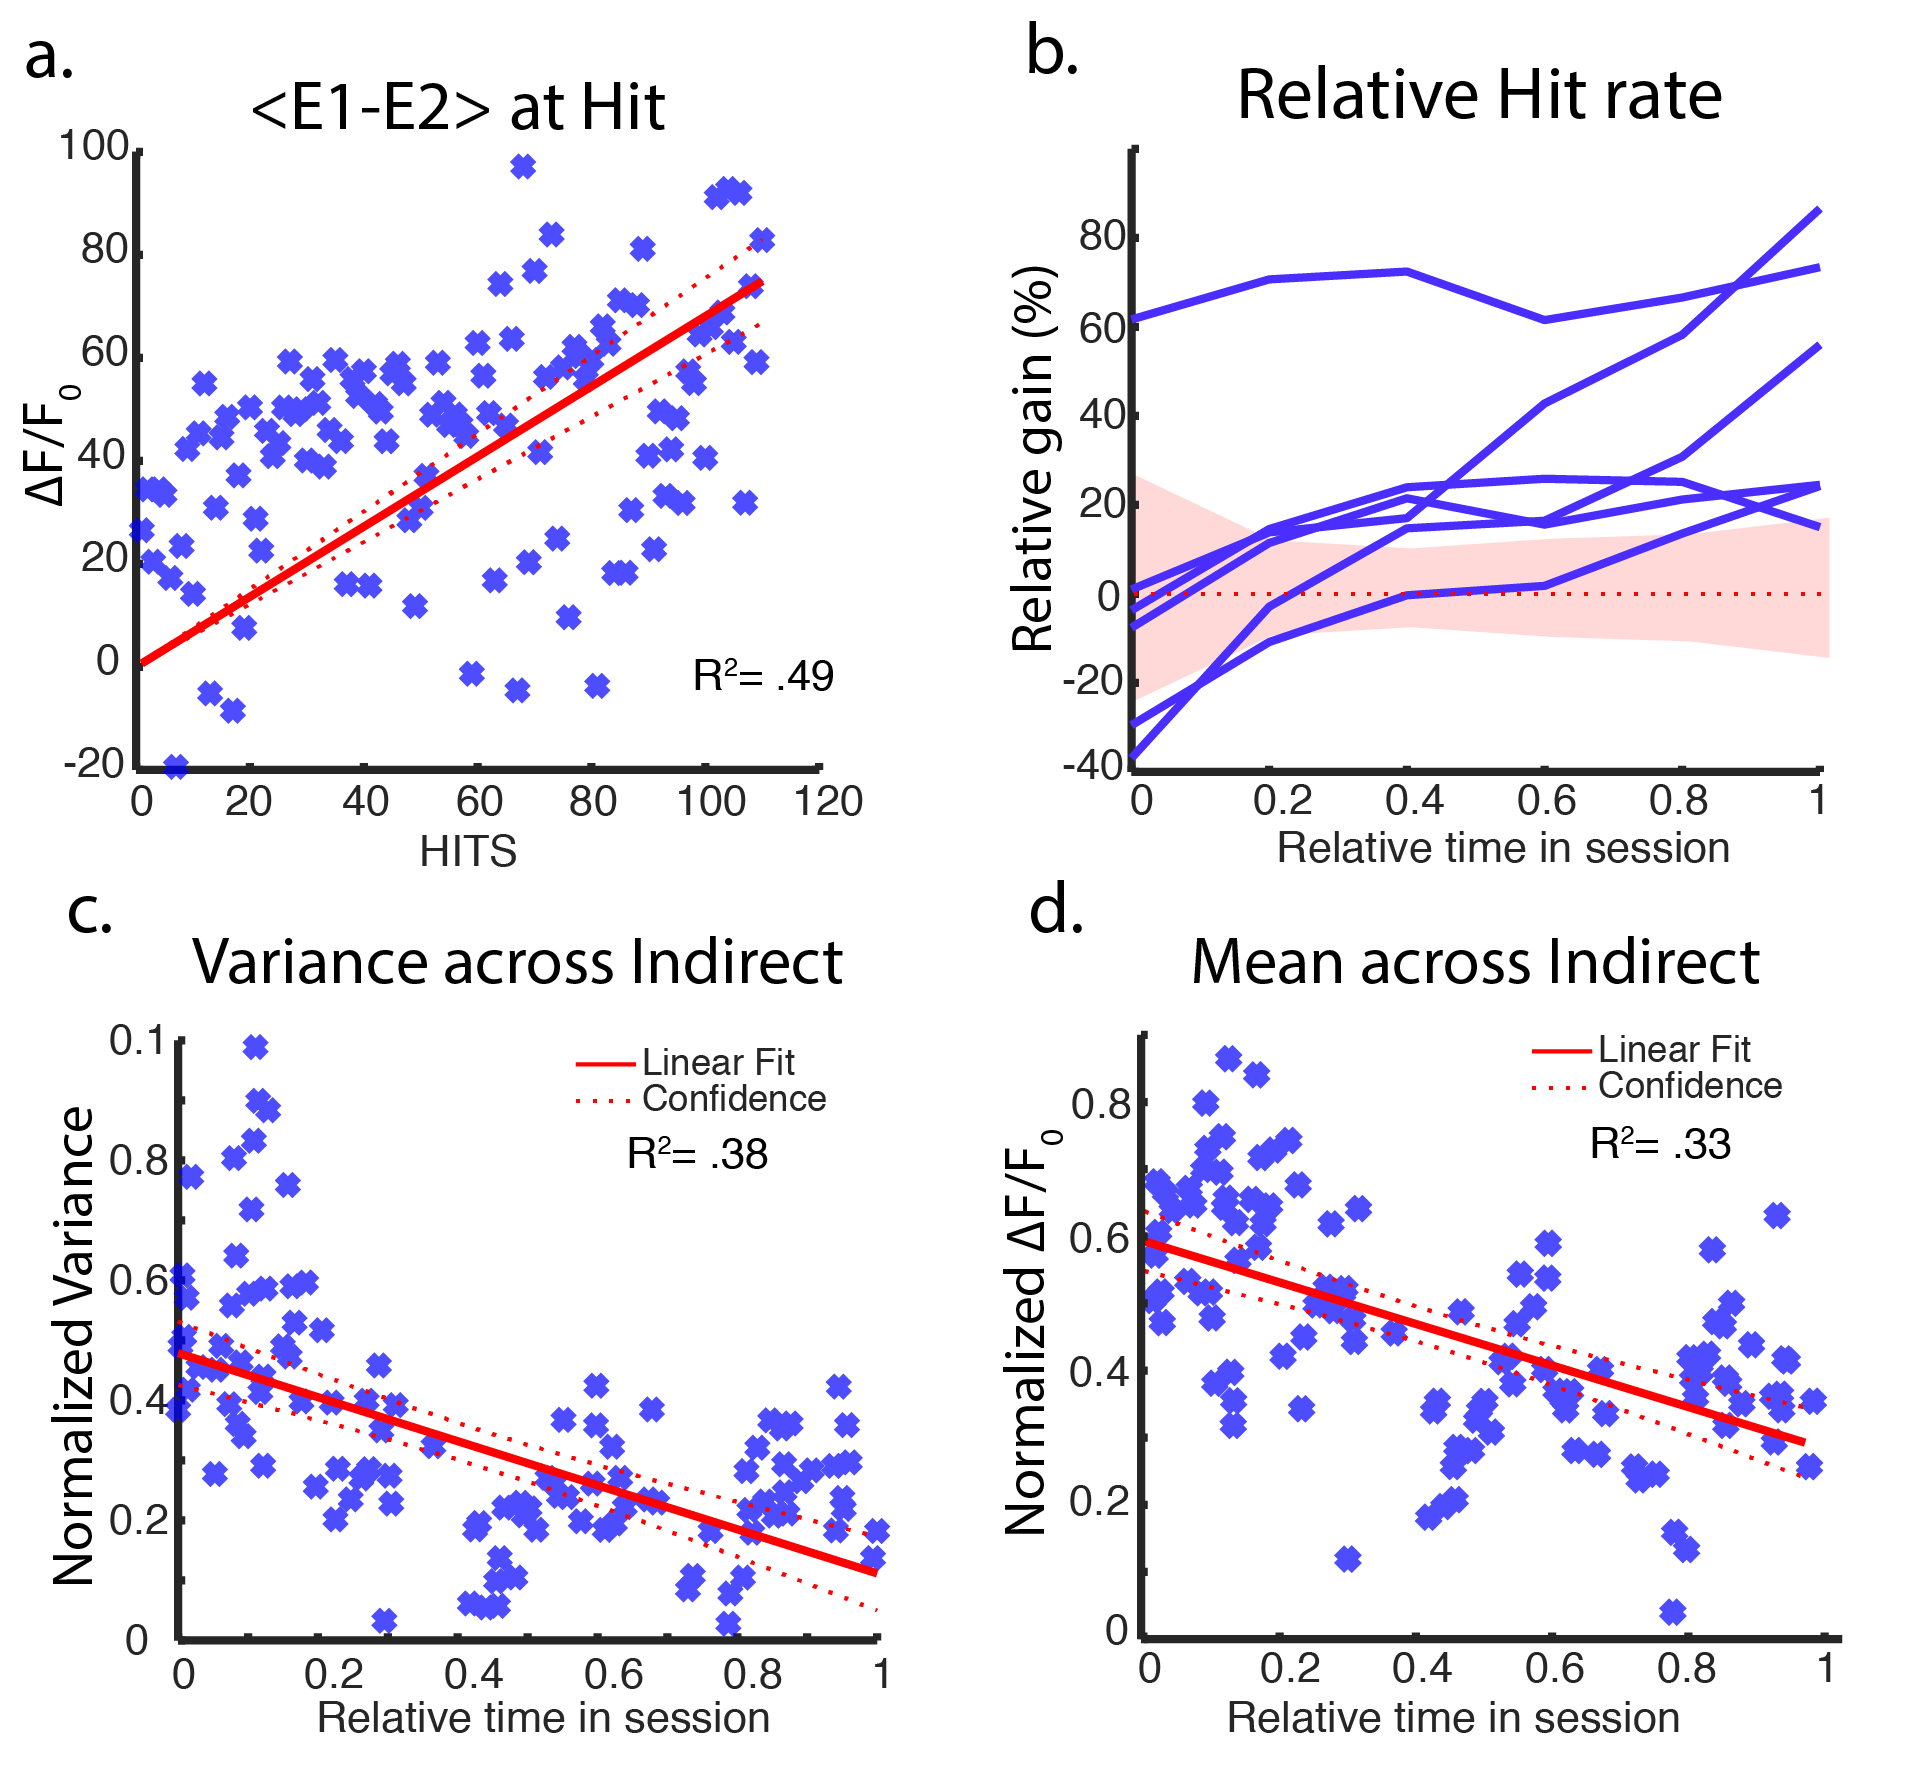
\includegraphics[scale=.52]{figures/figure02.png}
      \caption{\emph{Unrewarded neural population activity patterns sparsen over time.} $(A)$ Relative $\Delta F/F_{0}$  of the output neurons, significantly increases throughout the course of the session ( p$<$0.01). $(B)$ Compared to the simulated rate of reward using random pairs of indirect neurons, we find there is a strong trend to increase reward related conformations over time.  Each blue line represents one animals across a single day of BMI training. The red line indicates the distribution of reward rates for all animals that would have been achieved if any other pairs of neurons had been driving the cursor ( shading is 2$\times sem$). $(D)$ For this same animal in $A$, variance across the population of indirect neurons within one second preceding the hit drops significantly across the session ( p$<$0.01), $(D)$ as does the mean $\Delta F/F_{0}$ across the this same interval ( p$<$0.01). Each blue marker is a sample taken at the 'hit'}
      \label{figurelabel}
   \end{figure}
  

\subsection{Prediction of Output Cells Using Indirect Neuron Activity}
Increase of the relative hit rate over time suggests that the network is learning to specifically modulate a subset of neurons to increase the reward rate (Fig 2b). We reasoned that it may be possible to observe network credit assignment by modeling how well the population is able to decode output neuron activity, relative to non-output related cells. Using L2-regularized linear regression (also known as ridge regression), we find that the direct neuron $\Delta F/F_{0}$ can accurately decoded from the indirect population activity with high accuracy ($R^2$ values for $E1\textsubscript{a}$ = 0.77, $E1\textsubscript{b}$ =  0.78,  $E2\textsubscript{a}$ = 0.71, $E2\textsubscript{b}$ =  0.53) in addition to the the ensemble activity ( $R^2$ E1 = 0.65,  E2 = 0.69). The cursor value was more difficult to decode ($R^2$ = 0.36), suggesting the indirect population encodes the motor output, rather than integrating incoming sensory information. We find that a subset of neurons (10-20\%) can decode the majority of the variance in the direct cells. This finding suggests that the network is able to learn to quickly identify and assign credit to specific output neurons to provide neuroprosthetic control. Moreover, we use the weights of the regression model to see which indirect cells care the most about the cursor/direct neurons. Interestingly, we find that these cells are sparsely distributed and not necessarily local to the direct neurons- even though previous reports have shown that indirect cells tend to weakly co-vary with nearby direct neurons,\cite{Sriram2018-qy,Hahnloser2002-uf}.


\subsection{Spatiotemporal Distribution of Indirect Cells }
The fact that a number of indirect neurons can be predicted by the population with similar accuracy as the direct neurons, but the relative diversity of network conformations is decreasing throughout the task,  suggests that this neuroprosthetic skill may be driven by spatiotemporal ensembles of many cells. Motor and premotor structures have been shown to be locally clustered when driving natural movement, which may result from intrinsic connectivity patterns \cite{Markowitz2015-xd,Georgopoulos2007-ct}. To test if this is true in our neuroprosthetic task,  for every successful ensemble configuration that satisfied the success criteria of a `hit', (ie. $E1-E2 > 2.5SD$), we take the activity 1.5s before and 1.5s after this moment, and observe how many cells have consistent changes in fluorescence across `hits'. We can compare the mean $\Delta F/F_{0}$ activity across a subset of hits for each indirect cell, and compared it to the mean ROI activity of an independent subset. ( eg, even vs odd  hits). We find that roughly 10-20\% this population form a temporal relationship with the direct neurons, and consistently either lead or follow the activity of output neurons(Fig 4a,c)\cite{Prsa2017-rn}. This result suggests that indirect neurons coordinate the timing of cells that directly drive the effector. Plotting the spatial distribution of these cells reveals striking spatial structure. (Fig 4b,d). 
   \begin{figure}[thpb]
      \centering
%      \framebox{\parbox{3in}{We suggest that you use a text box to insert a graphic (which is ideally a 300 dpi TIFF or EPS file, with all fonts embedded) because, in an document, this method is somewhat more stable than directly inserting a picture. }}
      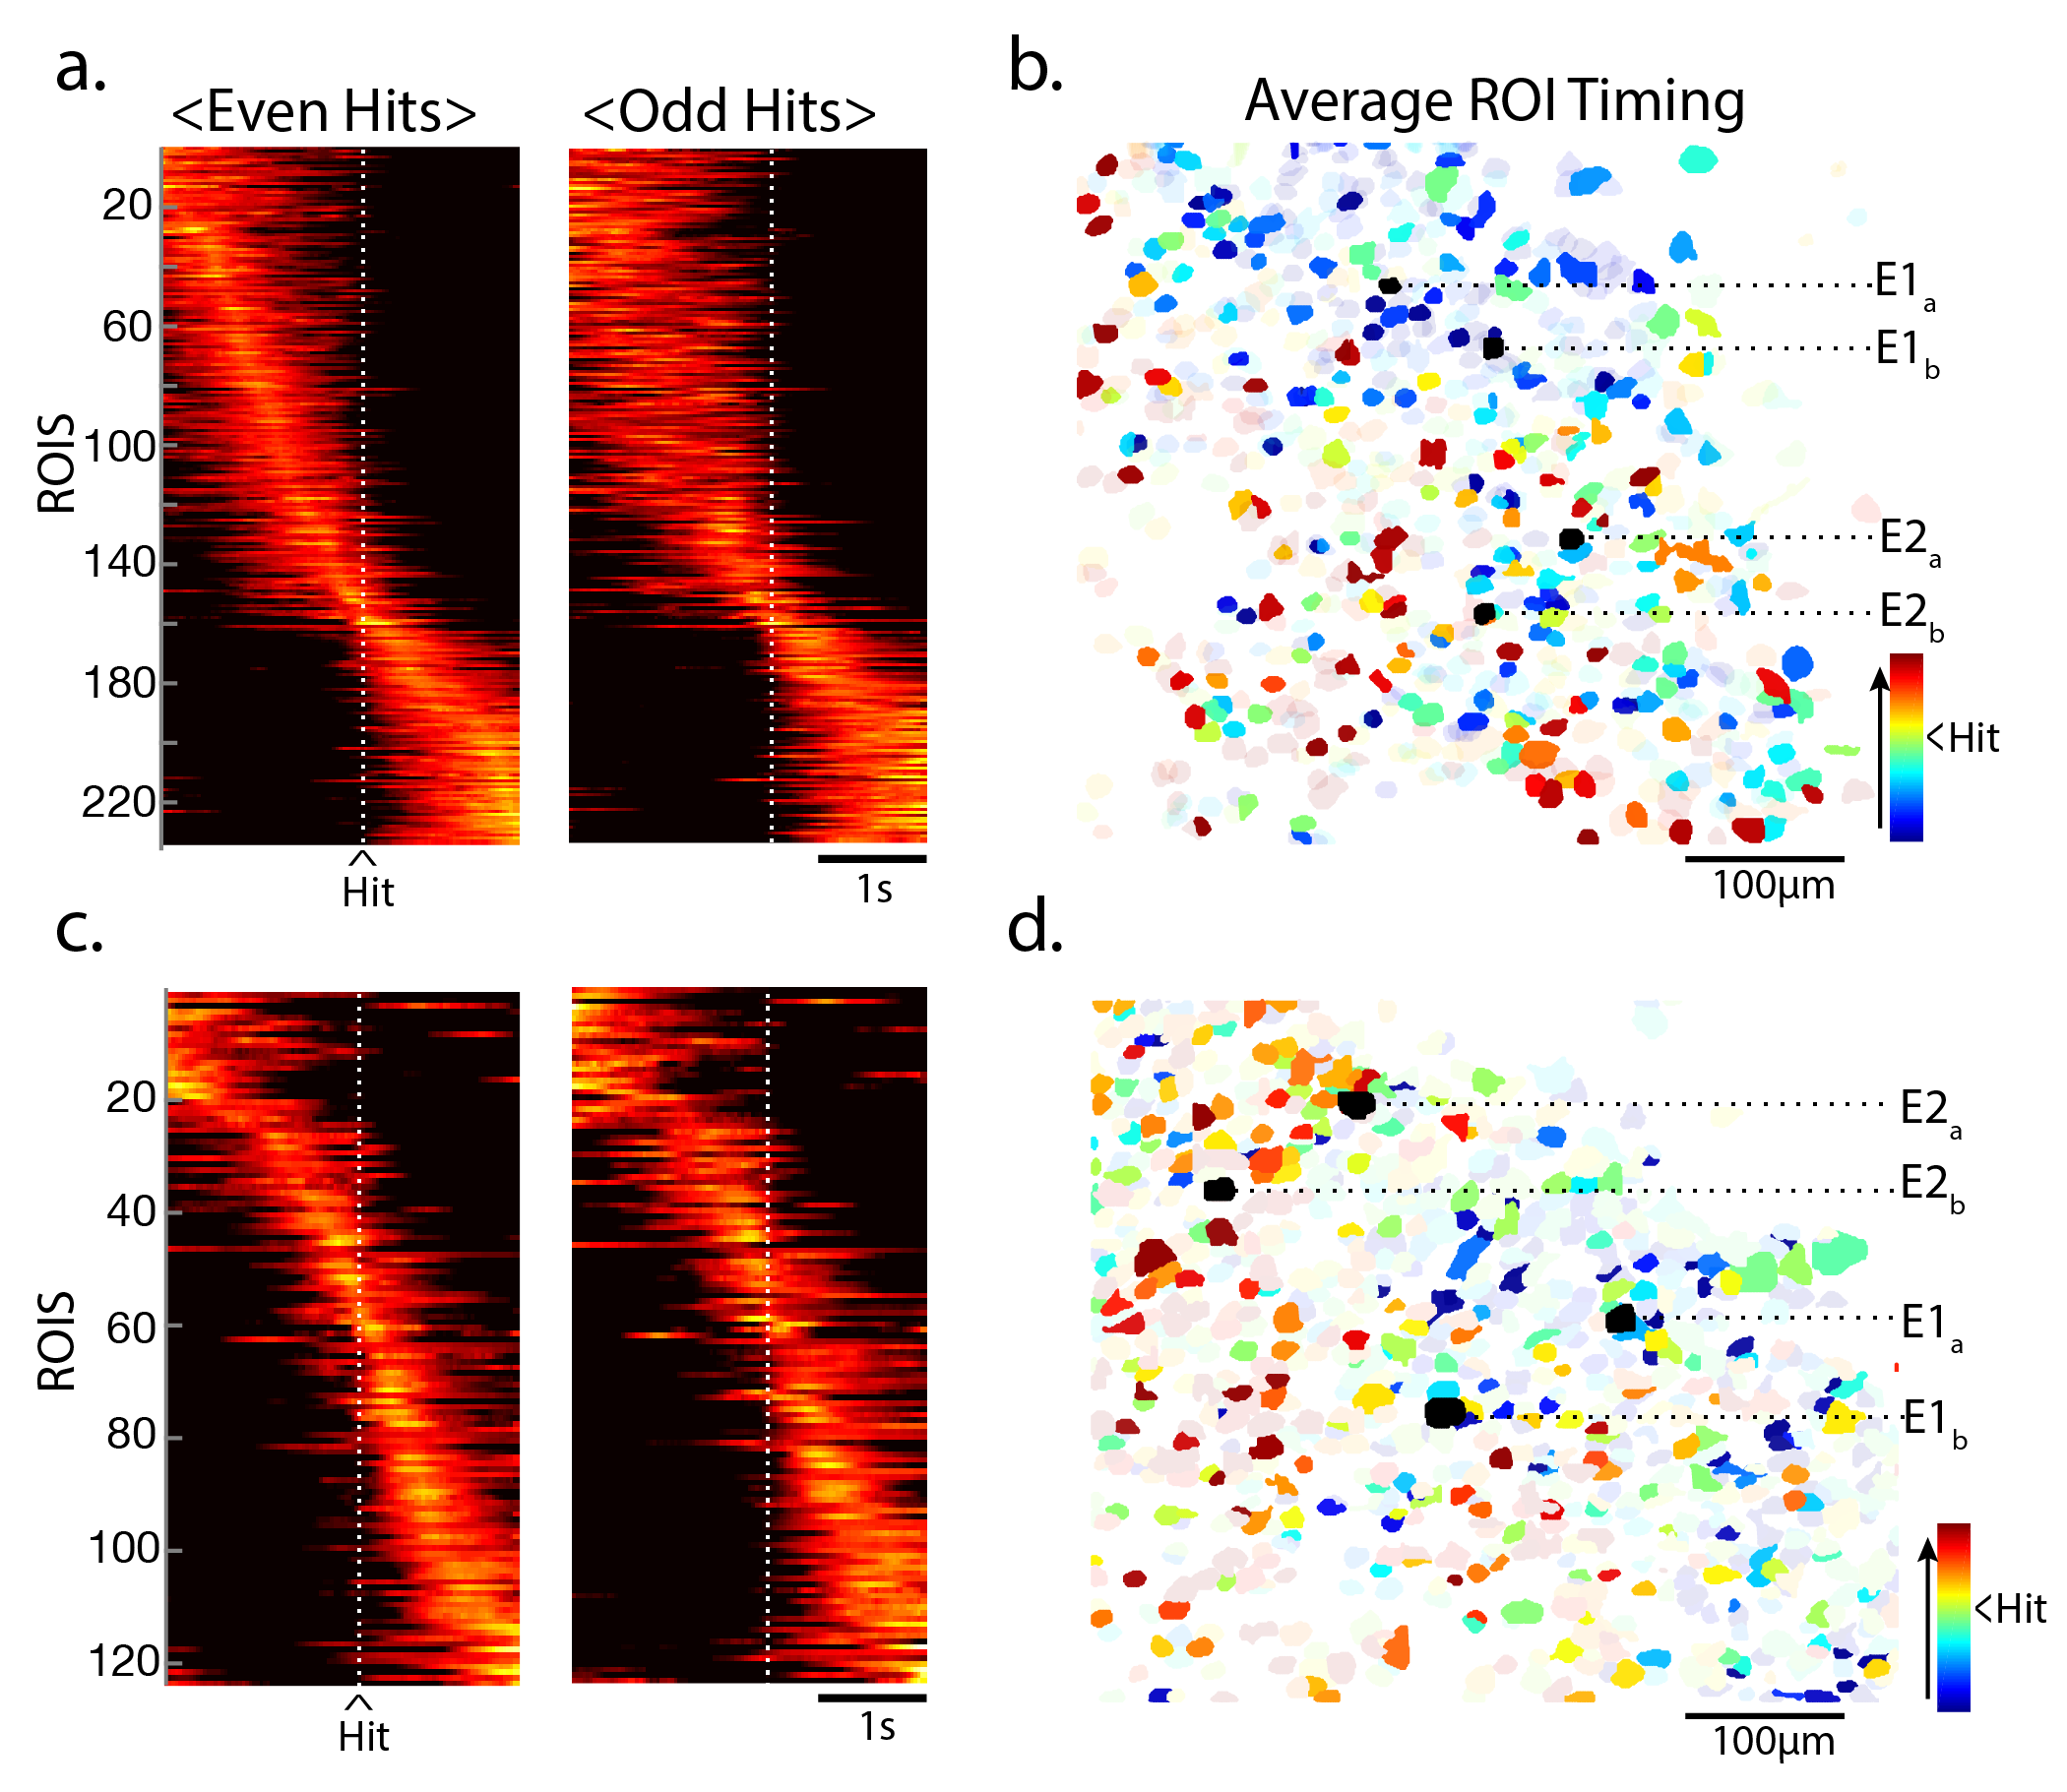
\includegraphics[scale=.50]{figures/figure03.png}
      \caption{\emph{Indirect neurons form robust spatiotemporal patterns leading up to, and following the rewarded output neuron configuration.} $(A)$ Three seconds of activity, centered at the reward criteria ('trials'), were split into two interleaved groups ( 55 each, 110 total for this animal) and averaged across trials. The mean ROI activity was sorted on the even trials, and this sorting is applied to the odd trials . A subset of ROIs demonstrated  high consistency ( right panel displays 220/790 identified ROIs that all have $>$0.95 Pearson correlation). and this correlated with peak amplitude ( p$<$.01)  $(B)$ Identified regions of interest colored by time according to the sorting on the even trials in $A$. ROIs with $<$0.95 correlations are displayed but masked with opacity. $(C-D)$. Same plot as $A-B$, but using data from a previous day of imaging in a nearby cell population, where different output neurons had been selected (displaying 120/500 ROIs, sorted on the even trials from this day).}
      \label{figurelabel}
   \end{figure}
   
   \section{DISCUSSION}
The findings described here largely recapitulate observations seen in across-day learning in both neuroprosthetic, and natural motor tasks: behavioral performance and the consistency neural responses tend to stabilize over time \cite{Gulati2017-rz}. In this report, we demonstrate explicit evidence that neuroprosthetic learning within a day can be the result of an initial increase, then rapid decrease of unrewarded neural activity patterns in neural populations that do not control an external effector. This result highlights a classic prediction from reinforcement learning theory: early in a session, there is high variance while the network explores various network conformations- those that lead to reward are consolidated and then exploited, and unrelated activity becomes sparse. It is important to note that neither the variance, or the individual performance seems to continue  decreasing by the end of the trial duration (30$min$) suggesting that this may be too short a window to master this particular task. In addition, we observe that the surrounding network can converge in space and time to produce repeated activity that is consistent on average. This suggests that ensembles of neurons, rather than individual cells, can act as the emergent functional unit of neuroprosthetic learning in mice \cite{Yuste2015-or}.  Possibly, this is the result of re-assigning endogenous existing sequences to achieve reward \cite{Golub2018-qc}.
 
The network spatiotemporal organization of motor cortex is unlikely to be predominantly sensory driven, given that neuroprosthetic skills show minimal modulation with passive tone playback \cite{Neely2018-ar} In conjunction, we observe that the indirect population cannot decode the tone ($R^2$ = 0.36) as well as the ensemble activity ( mean $R^2$ = 0.70), suggesting that the network can disambiguate reward expectation from reward guided behavior. Important caveats remain.  Wile previous work has shown that neuroprosthetic tasks operate without detectable behavior, it possible that motor consequences are sufficiently subtle and go undetected. 


\section{CONCLUSION}

Neuroprosthetic learning can be particularly insightful in studying the neural basis of sensorimotor integration. By explicitly constraining both the intrinsic jitter found in natural motor production, and the variability of performance evaluation, these experiments allow explicit measurements of how network patterns emerge to form behavior.

\addtolength{\textheight}{-12cm}   % This command serves to balance the column lengths
                                  % on the last page of the document manually. It shortens
                                  % the textheight of the last page by a suitable amount.
                                  % This command does not take effect until the next page
                                  % so it should come on the page before the last. Make
                                  % sure that you do not shorten the textheight too much.

%%%%%%%%%%%%%%%%%%%%%%%%%%%%%%%%%%%%%%%%%%%%%%%%%%%%%%%%%%%%%%%%%%%%%%%%%%%%%%%%



%%%%%%%%%%%%%%%%%%%%%%%%%%%%%%%%%%%%%%%%%%%%%%%%%%%%%%%%%%%%%%%%%%%%%%%%%%%%%%%%



%%%%%%%%%%%%%%%%%%%%%%%%%%%%%%%%%%%%%%%%%%%%%%%%%%%%%%%%%%%%%%%%%%%%%%%%%%%%%%%%
%\section*{APPENDIX}

%Appendixes should appear before the acknowledgment.

%\section*{ACKNOWLEDGMENT}

%Authors would like to thank to Wujie Zhang, Nick Dotson, David Piech, and Albert You and Ellen Zippi you for helpful discussions. 

%\begin{thebibliography}{99}

\bibliography{bib_short}{}
\bibliographystyle{IEEEtran}
%\bibliographystyle{unsrt}

%\end{thebibliography}




\end{document}




% bib
